\chapter{Implementation and Evaluation}
Based on the method we propose, we have implemented a search engine as well as a crawler and a parser for \LaTeX\ content. Also, a demo~\footnote{demo page: \url{http://infolab.ece.udel.edu:8912/cowpie/}} with Web interface is available for demonstration. 
In this chapter, we will introduce the way we implement our proposed method and use this system to evaluate its effectiveness and efficiency.

\section{System Overview}
Our system is consisted of a crawler, a parser, an indexer, a search program back-end and a Web front-end. 
The crawler searches and extracts math mode \LaTeX\ from Website that directly returns \LaTeX\ markup (e.g. from math content websites using client-side rendering, e.g. MathJax). The parser parses \LaTeX\ markup and prints the generated operation tree.
The indexer uses parser to transform \LaTeX\ markup into operation tree and indexes sub-paths on disk. 
The search program searches a query in index and returns search results, also exports a library for Web front-end which is a CGI program to interactive with user. 

The outline of our system process is, crawl and convert math expressions into an in-memory tree structure, then write the leaf-root path labels along with degree number associated with each nodes (we call \textit{branch word}) to disk as our index. 
When a user uses our Web front end to search, the Web CGI program calls the search library to search and score similar expressions in index, the search library outputs ranking results and Web CGI program rewrite them in HTML.

\section{Implementation}
Each component of our search engine is implemented as a separated module, the only way to interact with each module is by calling library API another module exposes, or by reading/writing to a plain text file. 
In this section, we will describe the implementation detail for each isolated module.

\subsection{Crawler}
The crawler is a python script using \textit{BeautifulSoup} to crawl Web pages and extract math mode \LaTeX. 
We have implemented a crawler specifically for the posts on Math Stack Exchange website, crawler can be specified to crawl posts by page or post ID.
For a post, the crawler searches the pattern of a \LaTeX\ inline or display mode text using regular expression. 
When a \LaTeX\ mode has been extracted, it is stripped with line feed and saved as plain text file one mode text per line and one file per post.

\subsection{Parser}
We are tokenizing math content using lexer generator \textit{flex} and have implemented a LALR parser generated from a set of grammar rules in \textit{GNU bison}, specifically for MathJax content in a subset of \LaTeX\ (those related to mathematics).
Our parser transforms a math formula into an in-memory operation tree (representing formula tree), as an intermediate step to extract the path labels, path ID, and degree numbers associated, for every leaf-root path from the tree. 
Our lexer omits all \LaTeX\ control sequences not matching any pattern of our defined tokens, most of them are considered unrelated to math formula semantics (environment statement, color, mbox etc.).

The complete grammar rules we use to parse \LaTeX\ math mode text is listed in Appendix~\ref{grammarRules}. 
The start rule \textit{doc} represents a \LaTeX\ math mode (either inline or display mode).
Sub-rules (lower case names in grammar rules) handle mathematical patterns such as addition/subtraction, modular, relation (e.g. equality, greater than, less than), factor, script, brackets etc. 
Tokens are using upper case names, the \textit{atom} rule represents a series of tokens that are mostly used as an atom unit in mathematical context (e.g. fraction, root, infinity). Other tokens are as part of some grammar rules.
The partial list of lexer tokens for our parser are listed in Appendix~\ref{lexerTokens}, the left field is escaped \LaTeX\ command string, the right field in curly brackets is the token that the left command mapped to.
Although enumerating \LaTeX\ math mode commands results in a long lexer list, we get a very simple grammar rules that is enough to handle most of our crawled data.

An example of an operation tree plain text output generated from our parser for math expression 
$ -b \pm \sqrt{b^2 - 4ac}$ is shown by figure~\ref{exout}.
Where every node is associated with five values: symbol value (meaningful only for leaf node), label value, node ID (indicated by ``\#''), degree of that node (indicated by ``*'') and the rank of a node (indicated by ``@'') in terms of its father node.
The node ID for a leaf will be used to identify the leaf-root path with respect to that leaf node, and the rank of child node will used to locate non-commutative tokens in a math expression.
The indexer later will choose some of these information from nodes along a leaf-root path to index the tree.

\begin{figure}
\begin{center}
\begin{verbatim}
   `--(ADD, ADD, #14, *2, @0)
       `--(NEG, NEG, #7, *1, @0)
       |   `--[`b', VAR, #1, *1, @0]
       `--(SQRT, SQRT, #13, *1, @1)
           `-(ADD, ADD, #12, *2, @0)
               |--(HANGER, HANGER, #9, *2, @0)
               |   |--(SUP_SCRIPT, SUP_SCRIPT, #8, *1, @0)
               |   |   `-[`2', NUM, #2, *1, @0]
               |   `-[`b', VAR, #3, *1, @1]
               `-(NEG, NEG, #11, *1, @1)
                   `-(TIMES, TIMES, #10, *3, @0)
                       |--[`4', NUM, #4, *1, @0]
                       |--[`a', VAR, #5, *1, @1]
                       `-[`c', VAR, #6, *1, @2]
\end{verbatim}
\end{center}
\caption{Example parser output}\label{exout}
\end{figure}

\subsection{Index}
The indexer writes the information extracted from parser into disk. 
There are two parts in our index, the first part uses native file system (for the sake of implementation simplicity) to store leaf-root path labels in directories from which our search engine can go level by level. 
Path ID, degree numbers, and also the formula ID generating that leaf-root path (we refer these three as \textit{branch word}) are stored in a ``posting" file at the directory corresponding to that branch word labels, 
e.g. the tree in figure~\ref{oprtreeExample} will result in indexing two directories: ./VAR/TIMES and ./VAR/ADD/TIMES. 
All the indexed branch words with path labels corresponding to directory ./VAR/TIMES/ are stored in the posting file of that directory, located at ./VAR/TIMES/posting.bin in this case.
Branch words in a posting file are ordered by their formula IDs to speed search (so we can merge two posting files with size $M$ and $N$ respectively, then find the branch words with same formula ID in $O(M\times N)$ time).
The second part of our index is a key-value database (using \textit{Kyoto Cabinet}) to map a formula ID to additional information for that formula (e.g. original markup, number of leaf-root paths $|T_d|$ and the URL on which the formula is crawled).

\subsection{Search program}
\label{se-and-rank}
The compromised substructure searching (described in section~\ref{se-method}) is used in our search engine to filter out likely isomorphic expressions in our index.
Searching is performed by simultaneously going from all the directories corresponding to the generated leaf-root paths of query formula tree,
to all their merged subdirectories. 
We keep traversing, at each level intersect the branch words (by their formula IDs) in the posting files from all the searching directories. 
The intersected formula IDs actually represent the trees in our search set $\bigcap_{a \in L} \mathcal{I}_{\Pi}(a)$.
Every document formula spotted in the search set is considered as a hit, we then apply \textproc{markAndCross} algorithm to get its symbolic similarity score with query formula
(using the branch word information indexed in posting file)
.
The search program uses our ranking tuple described in section~\ref{rankingTuple} to indicate the overall similarity and rank items in search results,
i.e. to decide whether one should be ranked higher than the other, first compare $s$, if equal, compare $f(d)$ and then $r$.
In addition, we use a min-heap to keep the top-$k$ scored items in our search results (by replacing the lowest scored items if we find a newer hit with higher score), where $k$ is the maximum number of items we keep in search results.
We also place a early termination valve on the number of branch words can be searched for one query at a time,
so that when exceeding this limit, search engine will stop and return the search results it has up to that time. Because some query can potentially have a very long posting list, doing so would make our searching response time no more than a certain value.

\begin{figure}
\begin{minipage}[b]{2.65in}
\begin{center}
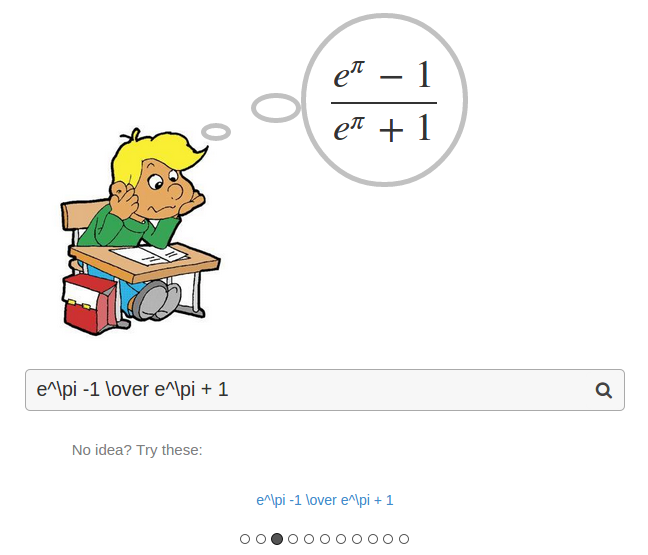
\includegraphics[height=2.5in]{se-page}
Search page
\end{center}
\end{minipage}
\hspace*{.38in}
\begin{minipage}[b]{2.65in}
\begin{center}
\raisebox{.0in}{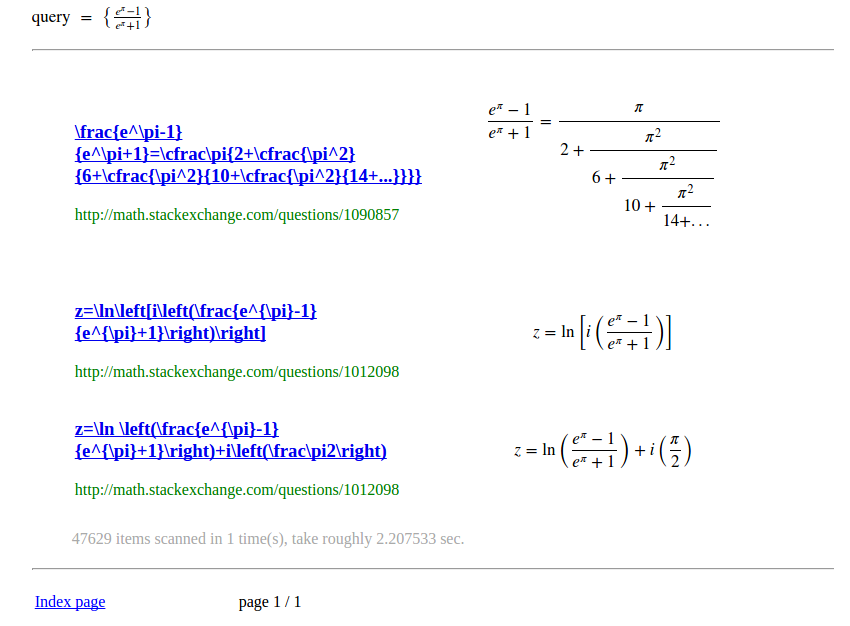
\includegraphics[height=2.5in]{res-page}}
Results page
\end{center}
\end{minipage}
\caption{Web front-end}\label{frontEnd}
\end{figure}

\subsection{Web front-end}
The Web front-end presents user a Web page (search page) that accepts a query in an input box and returns search results in several Web pages (result pages). 
User query is sent from browser to the front-end program by HTTP POST method and the start page of all ranked hits is specified by HTTP GET request.
The front end CGI program calls search library and wrap search results in HTML list elements, at the same time creates navigation links to help user browse results by page.
Figure~\ref{frontEnd} shows a screenshot of the search page and a result page from Web front-end.

\begin{table*}
\begin{center}
\renewcommand{\arraystretch}{1.5}
\begin{tabular}{|c|c||c|c|}\hline
ID & formula & ID & formula \\ \thickhline
1 & 
$\int_0^\infty dx \int_{x}^\infty F(x,y)dy  =\int_0^\infty dy \int_{0}^y F(x,y)dx$ &
2 & 
$X(i\omega)$ \\\hline

3 & 
$x^n + y^n=z^n$ &
4 & 
$\int^{\infty}_{-\infty} e^{-x^2} dx$ \\\hline

5 & 
$\frac{f(x+h)-f(x)}{h}$ &
6 & 
$\frac {\sin x} x$ \\\hline

7 & 
$ax^2 + bx +c$ &
8 & 
$\frac {e^x + y}{z}$ \\\hline

9 & 
$O(n \log n)$ &
10 & 
$H^n(X) = Z^n (X) / B^n(X)$ \\\hline

11 & 
$A_n = \frac 1 \pi \int_{-\pi}^\pi F(x) \cos(nx) dx$ &
12 & 
$\lim_{x \to \infty} (1 + \dfrac 1x)^x$ \\\hline

13 & 
$f(x) = f(0) + f'(0)x + \frac{f''(0)}{2!} x^2 + \ldots$ &
14 & 
$f(a) = \frac 1 {2 \pi i} \oint_r \frac{f(z)}{z-a} \;\mathrm{d}z$ \\\hline

15 & 
$x^2 + 2xy + y^2 = |x|^2 + 2|x||y| + |y| ^2$ &
16 & 
$\int_a^b f(x) \;\mathrm{d}x = F(b) - F(a)$ \\\hline

17 & 
$\frac {n!}{r_1! \cdot r_2! \cdots r_k!}$ &
18 & 
$-b \pm \sqrt{b^2 - 4ac}$ \\\hline

19 & 
$1+\tan^2 \theta = \sec^2 \theta$ &
20 & 
$\bar{u} = (x,y,z)$ \\\hline

\end{tabular}
\renewcommand{\arraystretch}{1}
\end{center}
\caption{Test query set}\label{TestQ}
\end{table*}

\section{Evaluation}
We rely on the search engine described in previous section to evaluate our search methods proposed in this paper.
Yet retrieval based on an equation is a relatively new task, previously studied in the context of NTCIR Math Tasks. 
The criteria to give judges about assessing the level of similarity degree between math expressions is not in a high level of agreement.
Nevertheless, we choose to evaluate our system by comparison to a naive baseline, and provide our intuitive guidelines for relevance judgements, given the newness of the domain.

\subsection{Dataset and index}
Our own dataset is created to evaluate proposed method.
We have crawled \LaTeX\ content from the posts of nearly entire (27180 pages of questions) Math Stack Exchange website before March 2015. 
The data set~\footnote{raw data: \url{http://infolab.ece.udel.edu:8912/cowpie/raw.tar.bz2} }
is plain text files generated by crawler output (\LaTeX\ math mode content per line, one file for each post).  
Over 8 million expressions of math mode are contained in the data set. 
The dataset is available through a roughly 60MB \textit{bzip2} compressed file.

Our test query set~\footnote{query set: \url{http://infolab.ece.udel.edu:8912/cowpie/test-queries.tex}} 
consists queries mostly from \cite{ntcirtopic} and \cite{symbolpairs15}, some of them are excluded here because we are unable to find similar formula in our own dataset.
Table~\ref{TestQ} shows our complete test queries used in our evaluation. 

The popular evaluation dataset in this research domain, the NTCIR Math Task collection, is in MathML/XML format, and original \LaTeX\ information is not always preserved in their dataset. 
Here we choose not to use their dataset because we are parsing \LaTeX\ directly.
Although converting MathML/XML formula to \LaTeX\ is possible, we fail to convert all the document in NTCIR dataset correctly (using \textit{pandoc}).
Furthermore, supporting wildcard query is a default requirement in NTCIR Math Task, while our approach does not support wildcard (see section~\ref{symSimi}).

After parsing our dataset using the indexer, the resulting index includes an 892 MB key-value database file and roughly 9.4GB directories and posting files.

\subsection{Relevance judgement}
We have defined four relevance levels, scored from 0 to 4 in our evaluation experiment.
This criteria considers both structural similarity and symbolic similarity. 
Structural similarity is scored by either 0, 1 (mostly similar) or 2 (complete matching);
symbolic similarity is scored by 0, 1 (mostly identical symbols for the matching parts) or 2 (identical symbols for the matching parts).
The level of relevance is simply the sum of the two scores.

\begin{figure}
\begin{minipage}[b]{2.65in}
\begin{center}
\begin{tabular}{|c"c|c|c|c|c|c|}
\hline
\multirow{2}{*}{Query} & \multicolumn{5}{c|}{Relevance Score} & \multirow{2}{*}{Judged} \\
\cline{2-6}
& 0 & 1 & 2 & 3 & 4 &   \\ \thickhline
1  &  15 &  2 &  2 &  0 &  1 &  20\\
2  &  20 &  0 &  0 &  0 &  0 &  20\\
3  &  15 &  4 &  1 &  0 &  0 &  20\\
4  &  0 &  0 &  0 &  6 &  14 &  20\\
5  &  0 &  0 &  0 &  8 &  12 &  20\\
6  &  0 &  2 &  5 &  2 &  11 &  20\\
7  &  1 &  4 &  3 &  3 &  9 &  20\\
8  &  4 &  2 &  13 &  1 &  0 &  20\\
9  &  17 &  2 &  1 &  0 &  0 &  20\\
10  &  5 &  1 &  1 &  1 &  0 &  8\\
11  &  0 &  0 &  4 &  11 &  5 &  20\\
12  &  0 &  0 &  1 &  16 &  3 &  20\\
13  &  0 &  0 &  0 &  1 &  6 &  7\\
14  &  0 &  0 &  4 &  13 &  3 &  20\\
15  &  14 &  3 &  1 &  1 &  1 &  20\\
16  &  0 &  2 &  5 &  8 &  5 &  20\\
17  &  0 &  0 &  0 &  15 &  5 &  20\\
18  &  8 &  6 &  2 &  2 &  2 &  20\\
19  &  0 &  0 &  5 &  13 &  2 &  20\\
20  &  19 &  1 &  0 &  0 &  0 &  20\\
\hline
\end{tabular}
\\[0.3cm] Baseline method
\end{center}
\end{minipage}
%%%%%%%%%%%%%%%%%%%%%%%%%%%
\hspace*{.38in}
%%%%%%%%%%%%%%%%%%%%%%%%%%%
\begin{minipage}[b]{2.65in}
\begin{center}
\begin{tabular}{|c"c|c|c|c|c|c|}
\hline
\multirow{2}{*}{Query} & \multicolumn{5}{c|}{Relevance Score} & \multirow{2}{*}{Judged} \\
\cline{2-6}
& 0 & 1 & 2 & 3 & 4 &   \\ \thickhline
1  &  13 &  2 &  2 &  1 &  1 &  19\\
2  &  15 &  1 &  0 &  3 &  1 &  20\\
3  &  0 &  0 &  0 &  0 &  20 &  20\\
4  &  0 &  0 &  0 &  1 &  19 &  20\\
5  &  0 &  0 &  0 &  0 &  20 &  20\\
6  &  1 &  0 &  0 &  0 &  19 &  20\\
7  &  0 &  0 &  0 &  0 &  20 &  20\\
8  &  4 &  3 &  12 &  1 &  0 &  20\\
9  &  0 &  0 &  0 &  0 &  20 &  20\\
10  &  4 &  1 &  1 &  1 &  0 &  7\\
11  &  0 &  0 &  4 &  11 &  5 &  20\\
12  &  0 &  0 &  0 &  9 &  11 &  20\\
13  &  0 &  0 &  0 &  1 &  6 &  7\\
14  &  0 &  0 &  9 &  6 &  5 &  20\\
15  &  14 &  2 &  1 &  1 &  2 &  20\\
16  &  0 &  0 &  0 &  0 &  20 &  20\\
17  &  0 &  0 &  0 &  14 &  6 &  20\\
18  &  0 &  0 &  2 &  0 &  18 &  20\\
19  &  0 &  0 &  0 &  0 &  20 &  20\\
20  &  0 &  0 &  2 &  7 &  11 &  20\\
\hline
\end{tabular}
\\[0.3cm] Similarity search
\end{center}
\end{minipage}
\caption{Relevance score distribution}\label{distrtab}
\end{figure}

\subsection{Results}
We have evaluated two methods here, a baseline method is a boolean search for structural related document using the method in section~\ref{se-method}; another method is a similarity search which further considers symbolic similarity score, matching depth factor and matching ratio as described in section~\ref{se-and-rank}.

Table~\ref{distrtab} shows the distribution of hits and relevance level for top 20 results (or less, if the number of hits are fewer than 20).
The performance and comparison of these two methods are shown in figure~\ref{perfcomp} and figure~\ref{effiperf}. 
The query look-up time is the time consumed for searching directories and posting files.
Results show that our similarity measurement, if used, can boost search effectiveness in all the five metres evaluated, 
and consumes a reasonable extra time on top of the baseline method. 

\section{Conclusion and Future Work}
Our method tries to measure math-expression similarity by their structures and operand symbols. 
We search structurally relevant expressions in a subset of index and our proposed similarity search method has achieved satisfactory effectiveness by our standard.
Meanwhile, our index does not need augmentation thus has less redundancy.
In the next stage, it is desired to integrate text search ability into our math-only search method. 
Additionally, the manner we use to break math formula into branch words and to index them through posting list make it easy to parallelize and distribute the searching process,
which means there is a large potential for future efforts to improve the efficiency of this method.

There are four levels of relevance scored from 0 to 4 in our evaluation.
The criteria considers both structural similarity and symbolic similarity. 
Structural similarity is measured by 0, 1 (mostly similar) and 2 (complete matching). 
While symbolic similarity is measured by 0, 1 (mostly similar for the matching parts) and 2 (identical symbols for the matching parts).
The level of relevance is simply the sum of the two scores.

directly huge
